\chapter{Resultados}
\label{resultados}

\section{PRIMEIRO TESTE}
\label{primeiro_teste}
O primeiro teste do projeto foi realizado na pista de atletismo da Unifor, no dia 8 de dezembro.
Logo ao chegar na pista de atletismos deparamos com o primeiro problema: a extensão não era grande o suficiente para atingir todo o percurso que escolhemos para treinar o Jaguar. Pedimos então aos auxiliares por uma nova extensão que foi entregue em pouco tempo. O jaguar foi treinado em apenas uma parte da pista, indo e voltando duas vezes. o Caminha percorrido é mostrado na figura \ref{pistaunifor}.

	\begin{figure}[H]
		\centering
		\Caption{\label{pistaunifor} Vista Aérea da Pista da Unifor}
		\UNIFORfig{}{
			\fbox{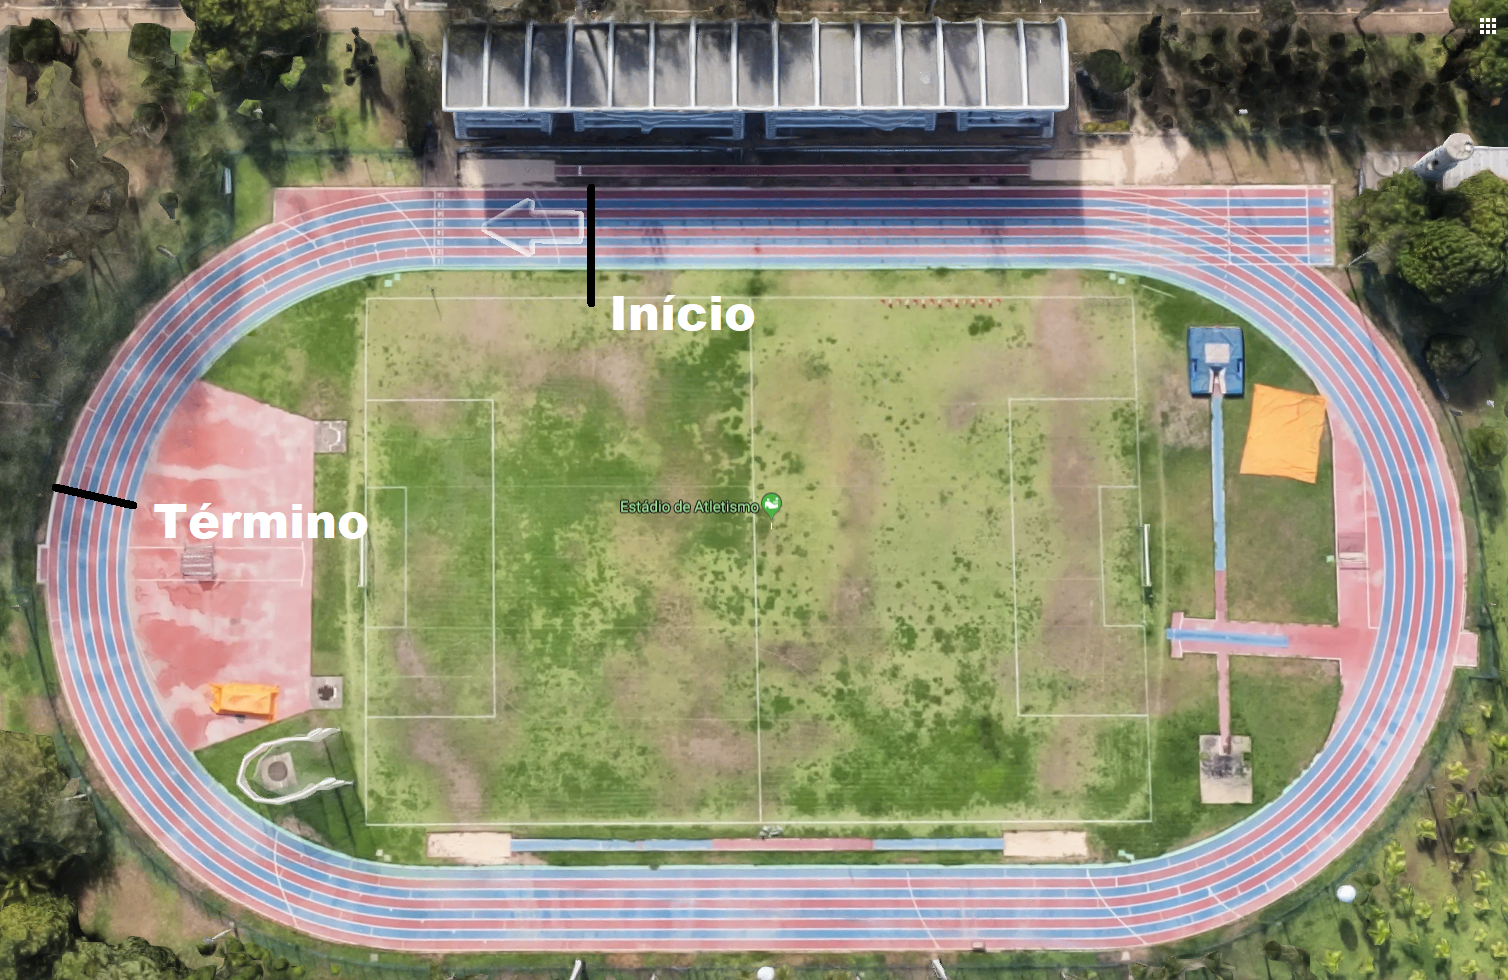
\includegraphics[width=16cm]{figuras/PistaUnifor.png}}
		}{
			\Fonte{\cite{pistaunifor}}
		}	
\end{figure}

Foram obtidas 977 imagens, o que ainda é muito pouco para criação de um modelo adequado para esse tipo de trabalho. Essas Imagens foram obtidas pela câmera do jaguar usando o programa \textit{savefile.py} enquanto um aluno pilotava o robô. As imagens são tiradas a cada movimento novo realizado no \textit{Joystick}. Na imagem \ref{jaguarelog} podemos ver a esquerda um exemplo de imagem capturada pela câmera do jaguar e a direta o resultado do terminal de execução do programa \textit{savefile.py}.

	\begin{figure}[H]
		\centering
		\Caption{\label{jaguarelog}Exemplo de Imagem capturada pelo câmera do Jaguar e o Terminal do programa \textit{Savefile.py}}
		\UNIFORfig{}{
			\fbox{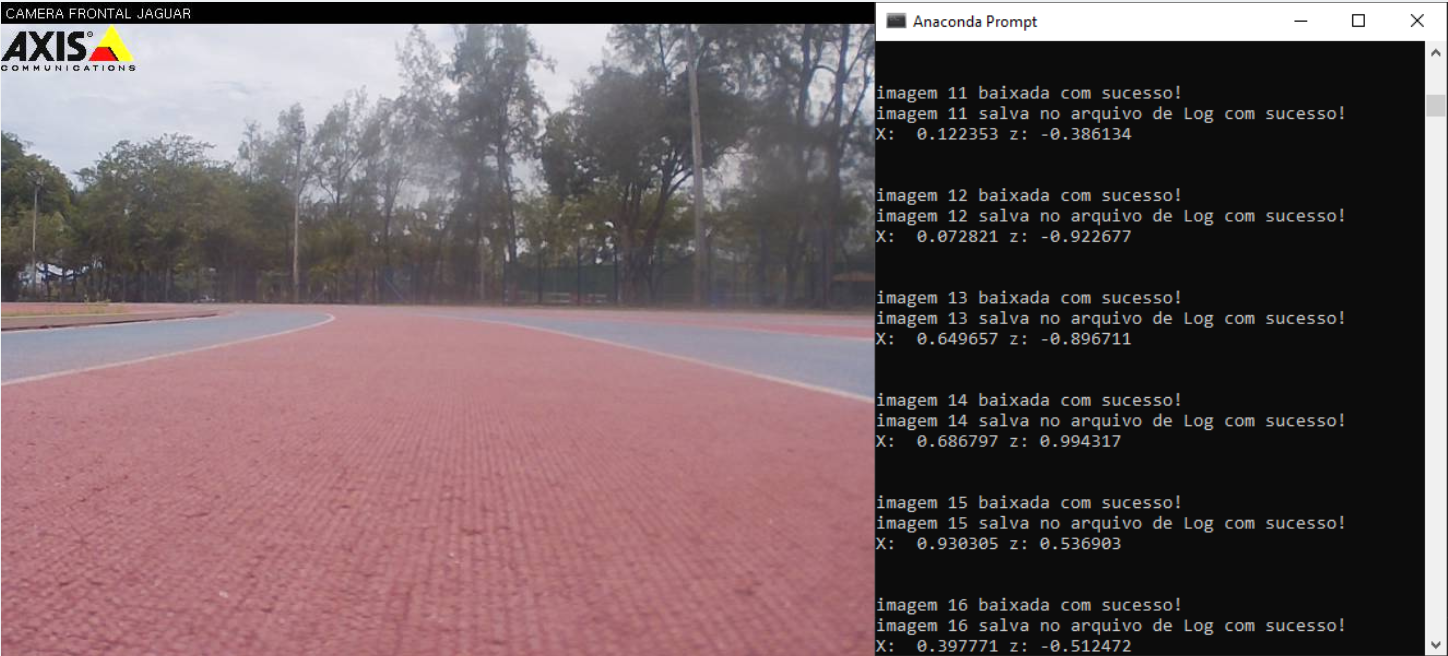
\includegraphics[width=16cm]{figuras/JaguarELog.png}}
		}{
			\Fonte{Elaborada pelo autor}
		}	
\end{figure}

O programa python tem acesso as imagens do Jaguar pelo IP de sua câmera. Ao final da captura das imagens, foi executado o programa \textit{model.py} que trata de criar o modelo de testes pro Jaguar, resultado no arquivo \textit{model-XXX.h5}, onde o "XXX" é o número do modelo da vez.

O programa \textit{model.py} tem o diretório com acesso a todas as imagens capturadas e o \textit{driver\_log} criado, caso não tenha sido mudado de lugar. Mas antes de criar o modelo, é feito um tratamento na imagem, com o auxílio o arquivo \textit{util.py}, para que seja processada com mais facilidade pela rede neural. Esse consiste em cortar o céu da imagem, que não será útil para o tratamento pela rede neural; reduzir o tamanho da imagem, o suficiente para ainda sim conseguir ser tratada pela rede neural e não perder nenhuma característica importante; por ultimo, muda as cores da imagem de rgb (o tradicional formato de imagem colorida) para yuv ( um formato mais simples de imagem utilizando menos cores e de processamento mais fácil).

Depois de tratada a imagem, é feito a criação dos modelos de rede neural, no qual o melhor será aquela com o menor \textit{val\_loss}. Para isso, é preciso modificar alguns parâmetros dentro do \textit{model.py}: \textit{np\_epoch} (defini o número de épocas de criação do modelo, ou seja, quantas vezes ele será treinado com aqueles padrões), \textit{sample\_per\_epoch} (quantidade de imagens por epoca) e \textit{batch\_size} (tamanho do lote de imagem de treinamento por vez). Normalmente a criação do modelo pode levar horas e exigir muito processamento do computador. Os parâmetros utilizado para cada treinamento estão na tabela \ref{parametros1}.

\begin{table}[H]
\centering
\caption{ Tabela de parâmetros do primeiro para primeira pista}
\label{parametros1}
\begin{tabular}{|l|l|l|l|}
\hline
\textbf{Treinamento} & \textbf{nb\_epoch} & \textbf{samples\_per\_epoch} & \textbf{batch\_size} \\ \hline
1º        & 5         & 5000                & 100         \\ 
2º        & 10        & 5000                & 100         \\ 
3º        & 5         & 10000               & 100         \\ 
4º        & 10        & 10000               & 100         \\ 
5º        & 15        & 10000               & 100         \\ 
6º        & 15        & 20000               & 150         \\ \hline
\end{tabular}
\end{table}

O \textit{model.py} está programado para criar o próximo modelo somente se houver um erro menor que o modelo anterior. As vezes ele cria somente um modelo pois o primeiro foi o melhor de todos, outras vezes ele cria vários modelos. Isso depende de cada caso.
No sábado seguinte, foi colocado para testar o último modelo criado, o \textit{model-009.h5} e, para a surpresa de todos, ele funcionou perfeitamente, sem a necessidade de testar nenhum outro modelo. Segue abaixo o valor do loss:

\begin{lstlisting}
loss: 0.0937 - val\_loss: 0.0564
\end{lstlisting}

Com o notebook conectado ao Jaguar, o Programa \textit{drive.py} foi executado juntamente com o \textit{model-009.h5} e, com apenas esse primeiro modelo, foi possível colocar a plataforma para percorrer a pista de atletismo nos dois sentido. A figura \ref{testejaguar} Mostra o teste realizado na pista no qual o notebook está no chão, ao lado robô.

	\begin{figure}[H]
		\centering
		\Caption{\label{testejaguar}Teste do Jaguar}
		\UNIFORfig{}{
			\fbox{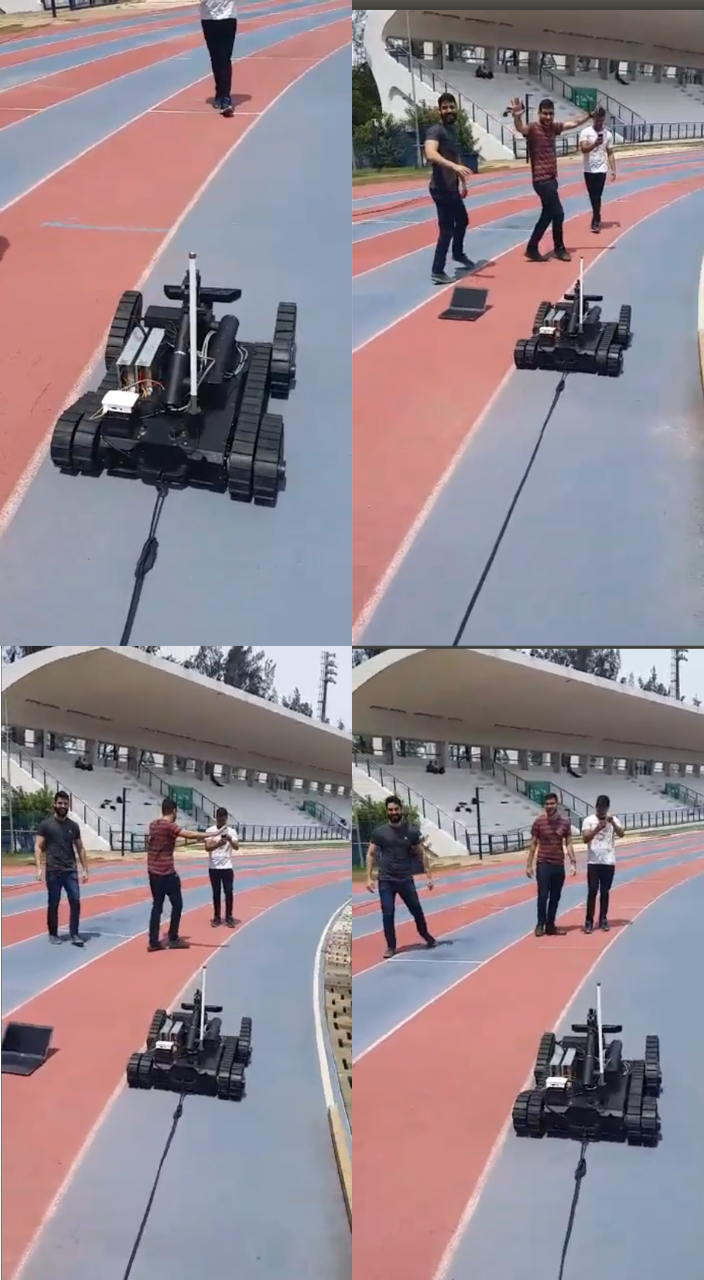
\includegraphics[width=16cm]{figuras/testejaguar.png}}
		}{
			\Fonte{Elaborado pelo autor}
		}	
\end{figure}


Em alguns momentos o Jaguar foi deslocado um pouco da sua rota. Mesmo assim ele consegue retornar a pista. Os resultados foram impressionantes, principalmente pelo fato das inúmeras limitações para o desenvolvimento do projeto.

\section{SEGUNDO TESTE}
\label{segundo}

Para validação do trabalho, é preciso que o Jaguar consiga treinar e percorrer em outros circuitos. O segundo teste foi feita na sala L4 com o formato de pista representado na figura \ref{circuito}:

	\begin{figure}[H]
		\centering
		\Caption{\label{circuito} Circuito da pista 2}
		\UNIFORfig{}{
			\fbox{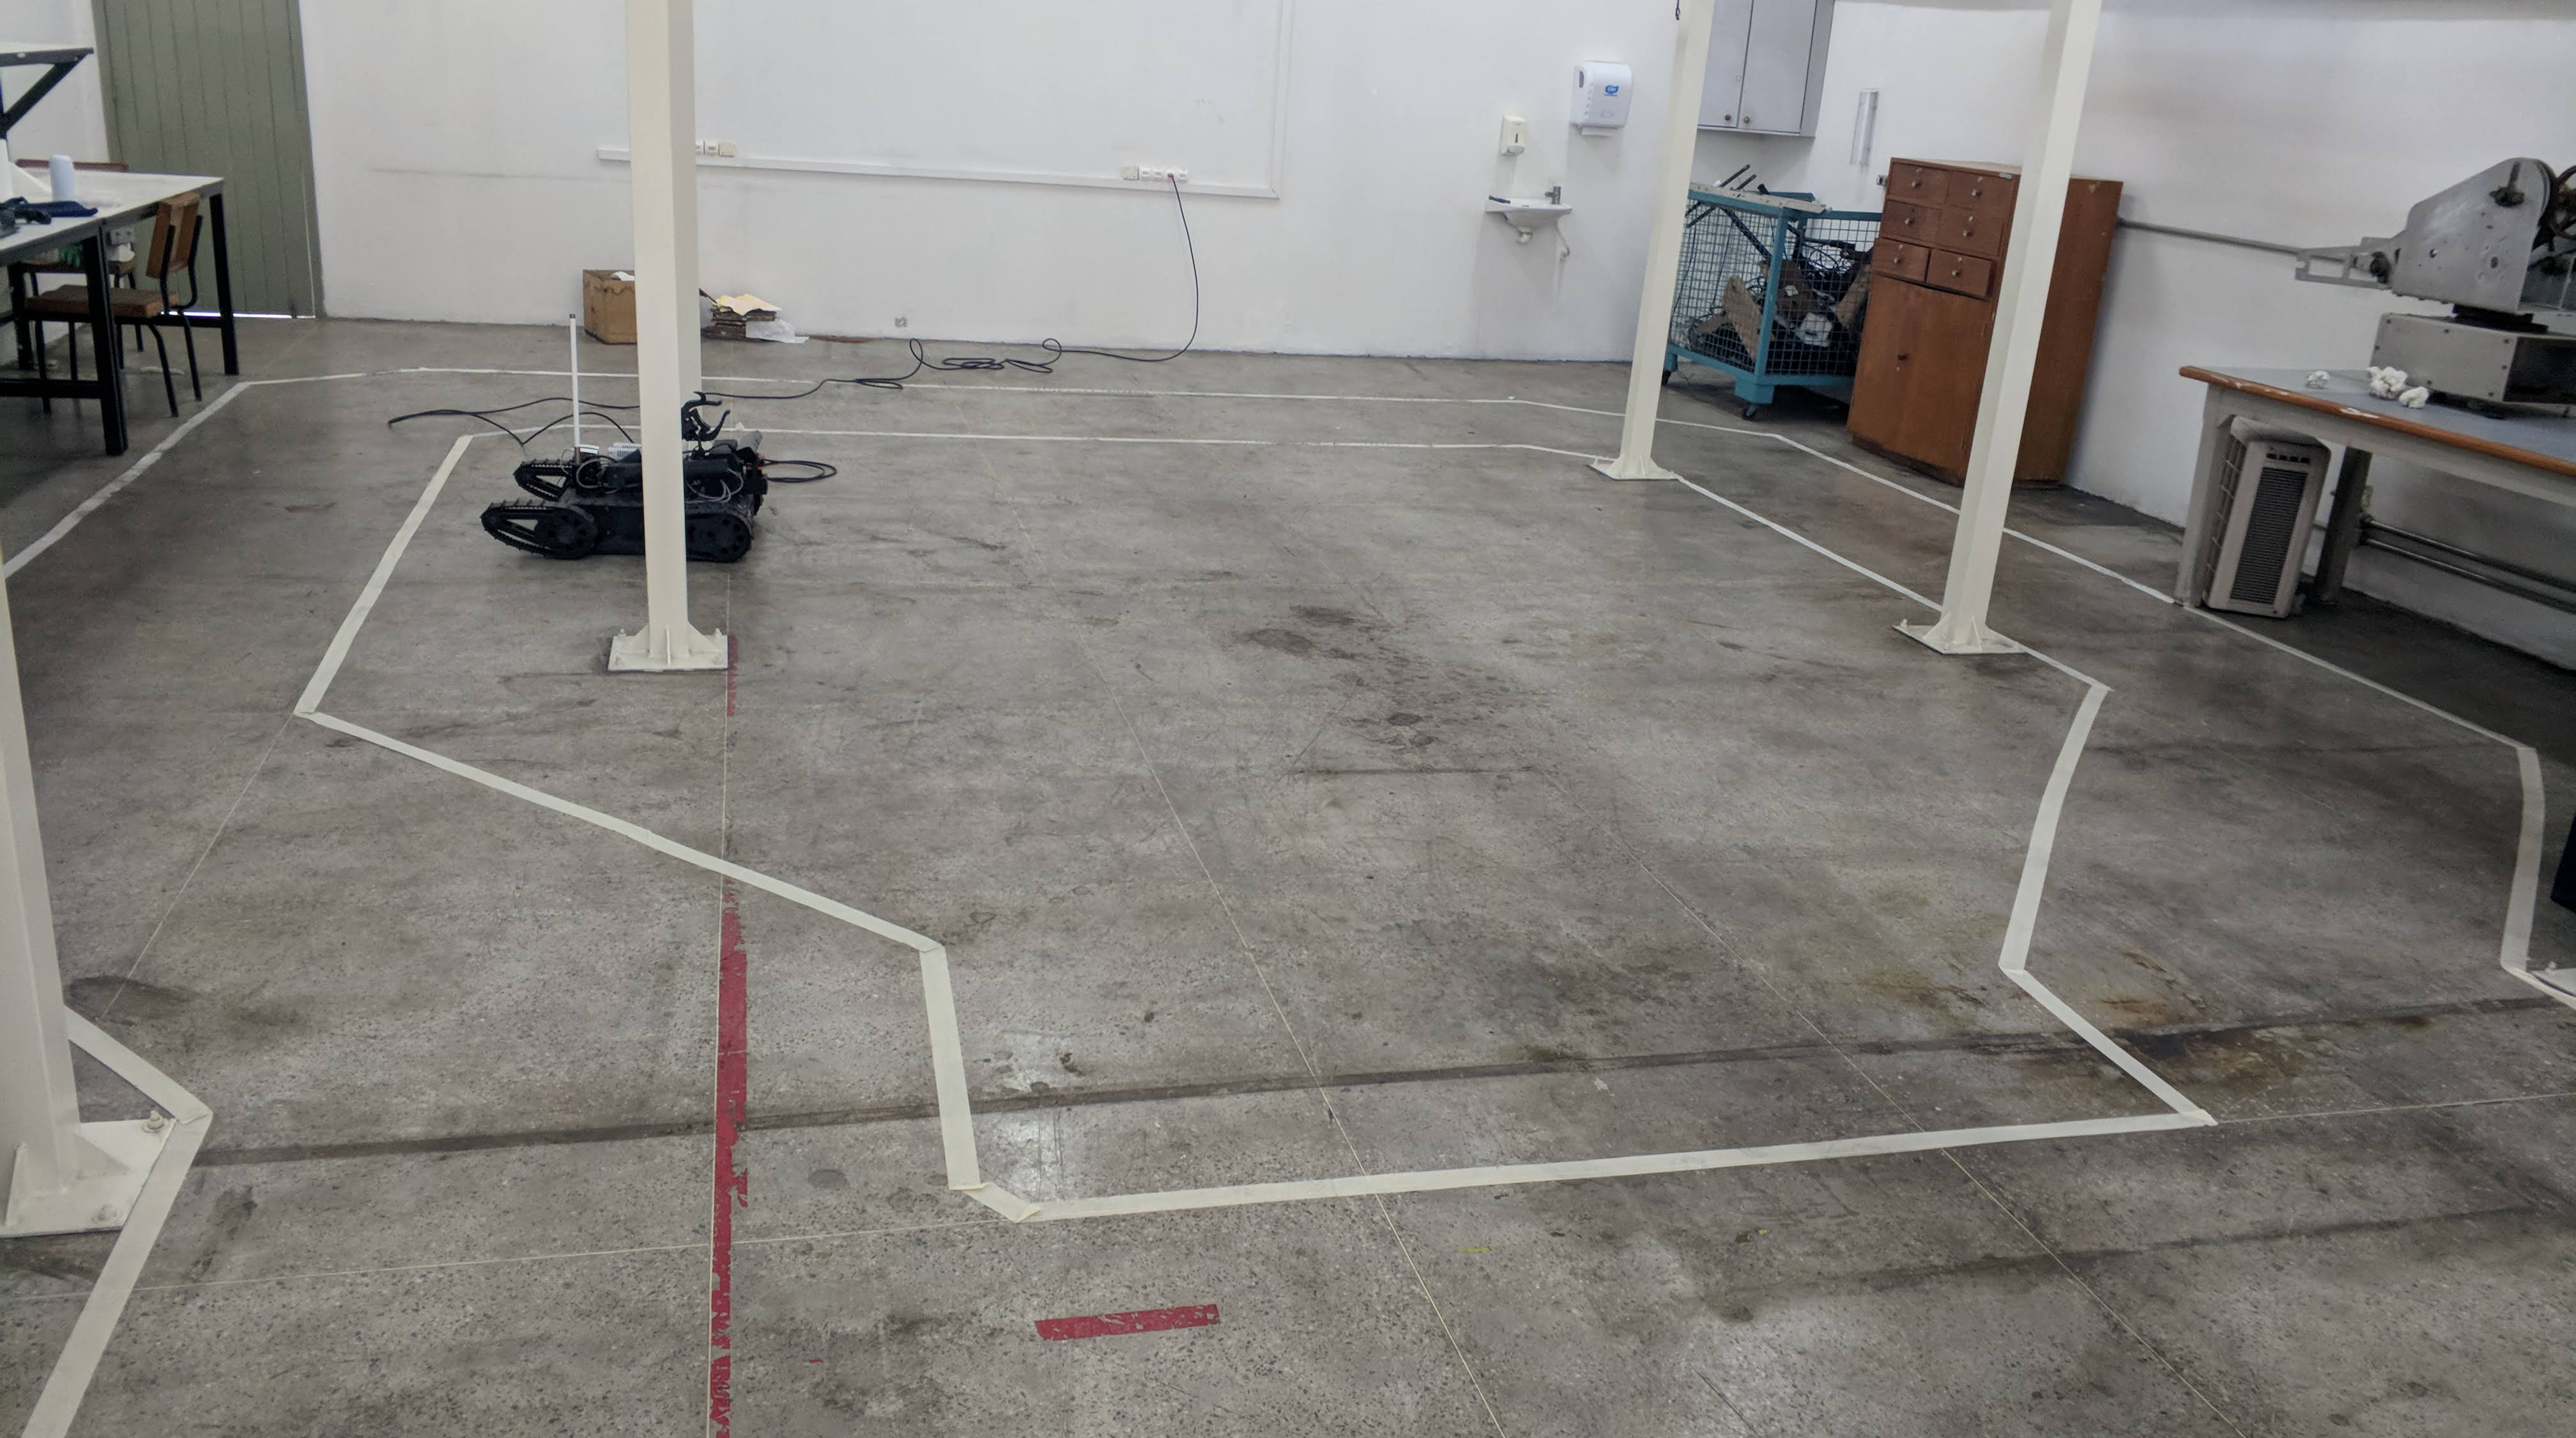
\includegraphics[width=15cm]{figuras/pista1.jpg}}
		}{
			\Fonte{Elaborado pelo autor}
		}	
\end{figure}

O segundo teste foi o mais trabalhoso. Ele foi realizado no laboratório L4 e a pista teve que ser refeita três vezes. A primeira foi a mais simples, feita de fita adesiva. Ela é mostrada na figura \ref{pista1}.

	\begin{figure}[H]
		\centering
		\Caption{\label{pista1} Primeira Pista da L4}
		\UNIFORfig{}{
			\fbox{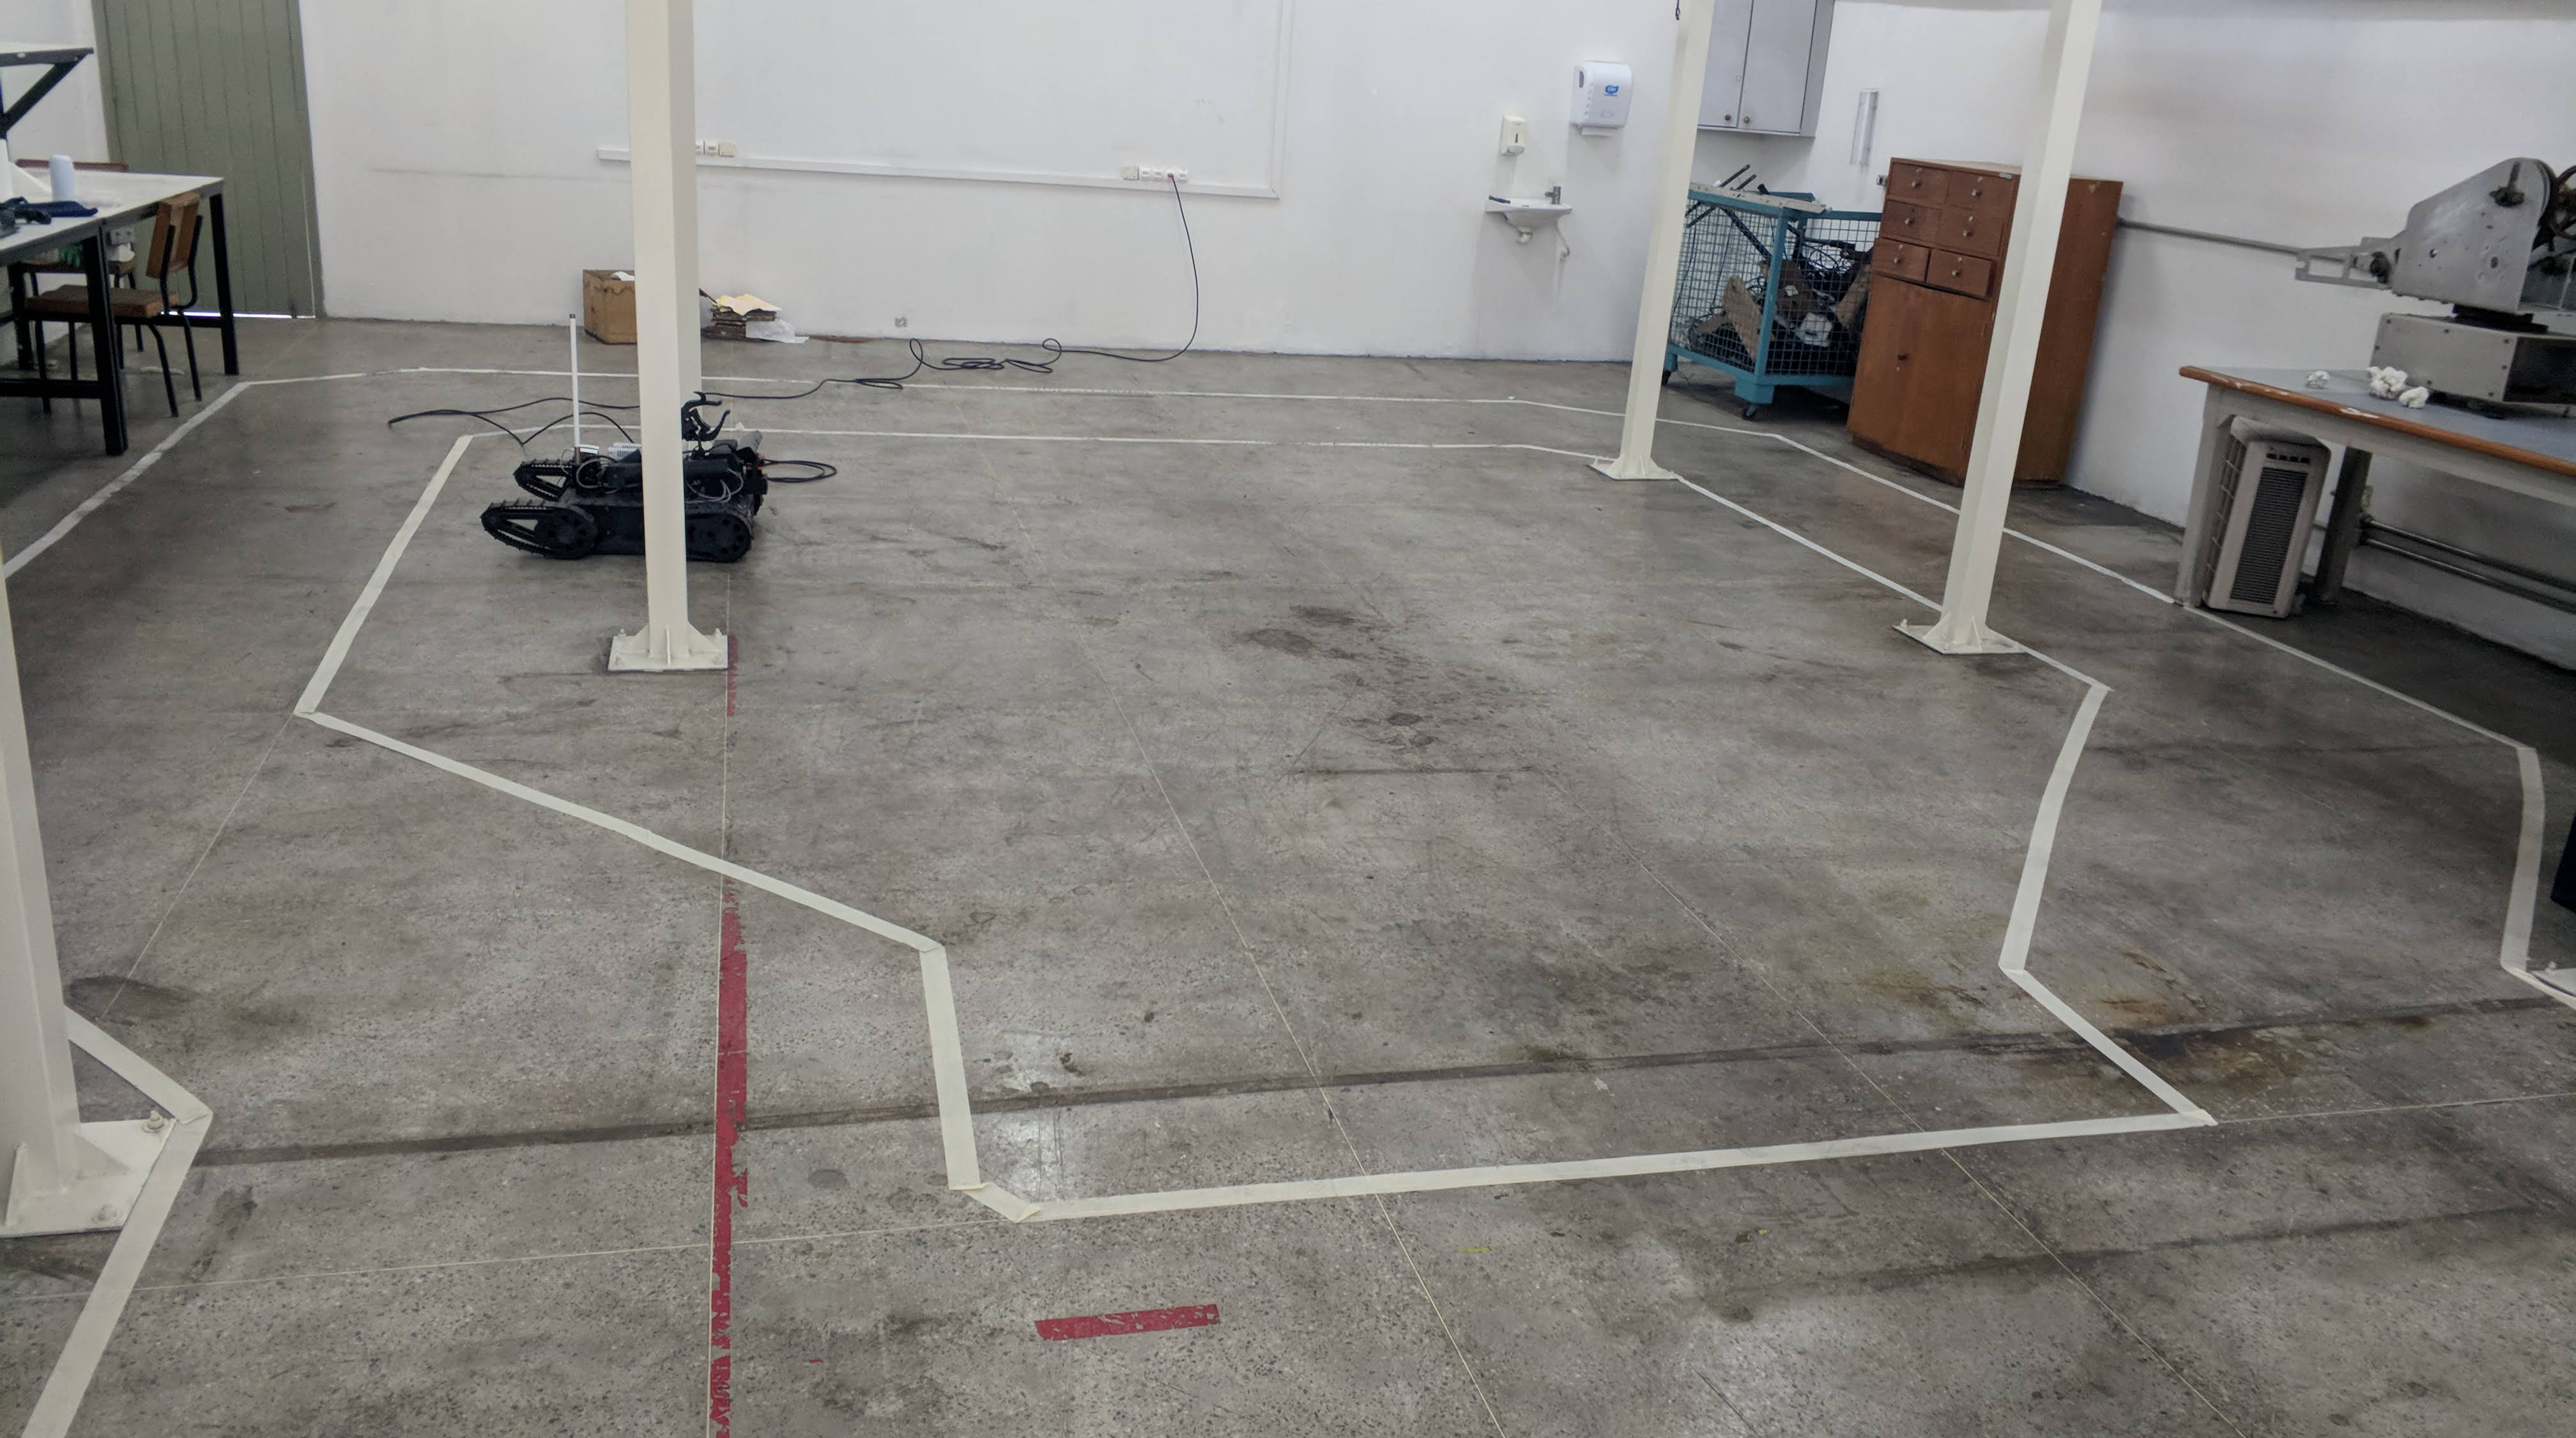
\includegraphics[width=15cm]{figuras/pista1.jpg}}
		}{
			\Fonte{Elaborado pelo autor}
		}	
\end{figure}

O primeiro grande desafio enfrentado foi desenhar um modelo de pista que Jaguar conseguisse visualizar. A fita adesiva, muito fina, não se destacava o suficiente no chão de cinza da L4. Mesmo com várias tentativas e vários modelos criados o Jaguar conseguia no máximo seguir por uma reta ou uma curva simples, mas logo se perdia. A imagem \ref{imagem1} mostra um exemplo de imagem capturada pelo Jaguar nessa pista.

	\begin{figure}[H]
		\centering
		\Caption{\label{imagem1} Imagem Capturada pela câmera do Jaguar}
		\UNIFORfig{}{
			\fbox{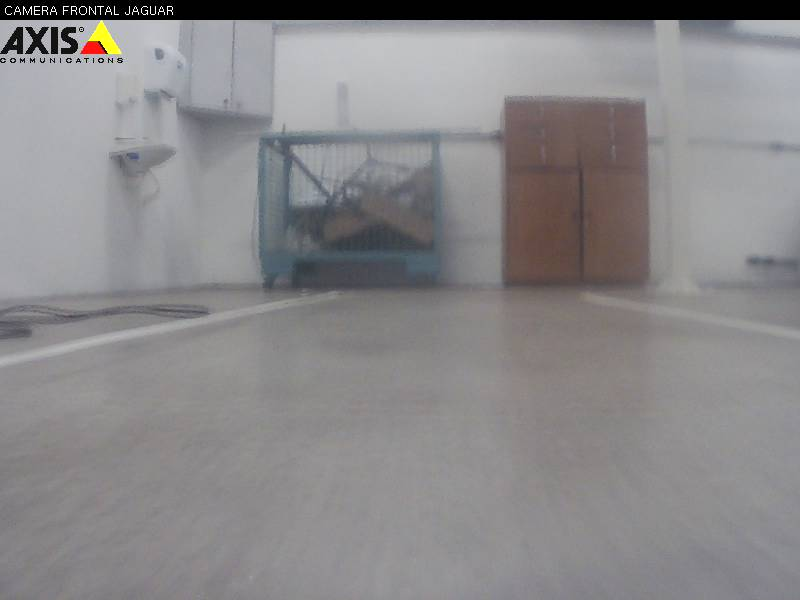
\includegraphics[width=15cm]{figuras/imagem1242.jpg}}
		}{
			\Fonte{Elaborado pelo autor}
		}	
\end{figure}


Mediante o problema de largura da pista, foi criado uma nova seguindo o mesmo modelo da anterior, porém com as bordas mais larga e feita de fita adesiva e papel toalha. Segue a pista na Figura \ref{pista2}:

	\begin{figure}[H]
		\centering
		\Caption{\label{pista2} Segunda Pista da L4}
		\UNIFORfig{}{
			\fbox{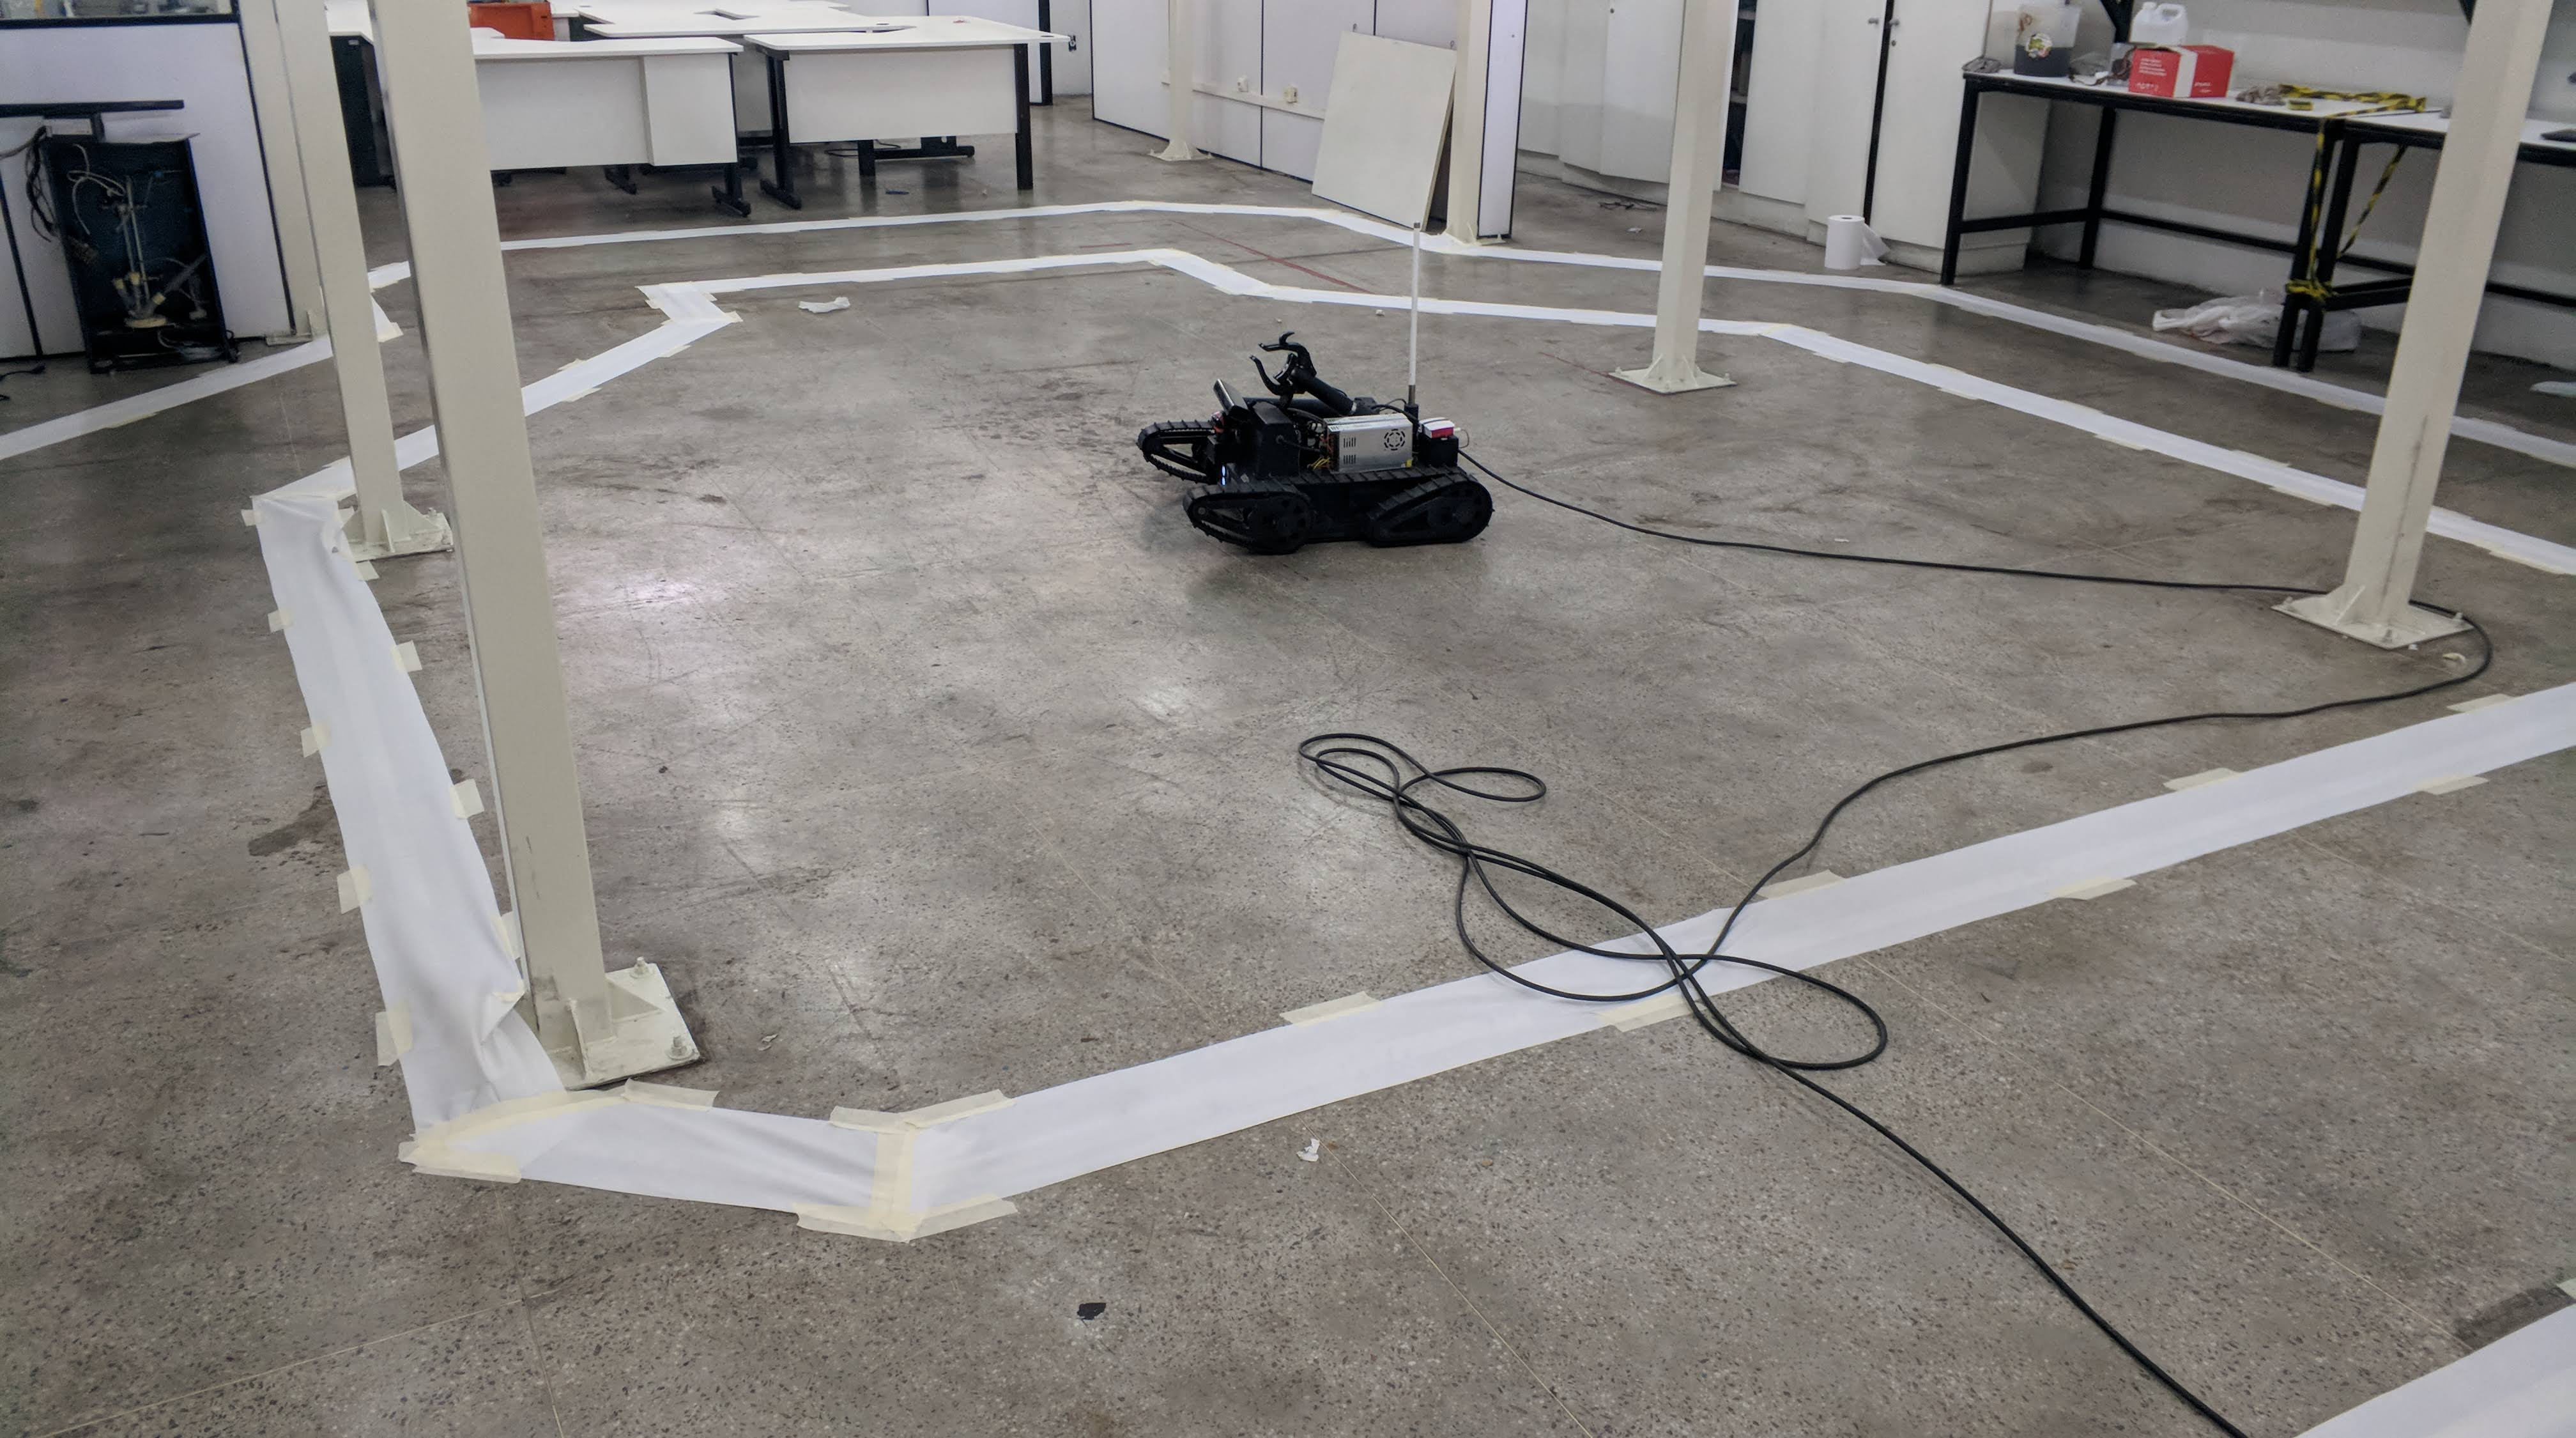
\includegraphics[width=15cm]{figuras/pis2.jpg}}
		}{
			\Fonte{Elaborado pelo autor}
		}	
\end{figure}


O grande problema da segunda pista foi o papel toalha. Toda vez que Jaguar errava alguma movimento e passava por cima da pista ele rasgava o papel toalha. Durante os testes e treinamento ela teve que ser refeita inúmeras vezes, mas pelo menos a segunda pista foi melhor para a visualização do Jaguar. 

	\begin{figure}[H]
		\centering
		\Caption{\label{imagem2} Imagem Capturada pela câmera do Jaguar}
		\UNIFORfig{}{
			\fbox{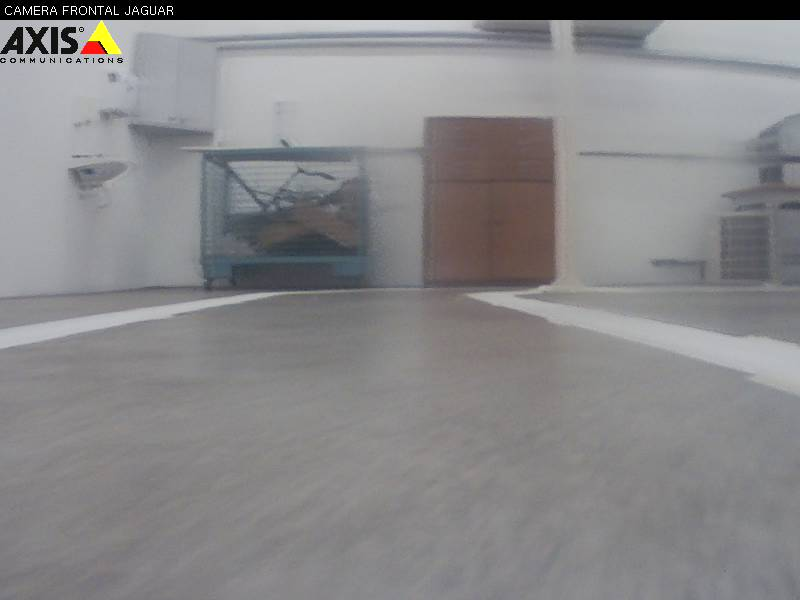
\includegraphics[width=15cm]{figuras/pista2imagemboa.jpg}}
		}{
			\Fonte{Elaborado pelo autor}
		}	
\end{figure}

A ultima pista foi feita do mesmo material da segunda, porém com a adição de fita zebrada amarelo e preta nas bordas da pista. Como o algoritmo visualiza melhor com uma grande diferença de cores, a fita deu um destaque na pista, facilitando para o processamento. A figura \ref{pista3} mostra a aplicação da fita zebrada nas bordas da pista e a figura \ref{imagem3} mostra a mesma pista sendo visualizada pelo câmera do Jaguar.

	\begin{figure}[H]
		\centering
		\Caption{\label{pista3} Ultima Pista da L4}
		\UNIFORfig{}{
			\fbox{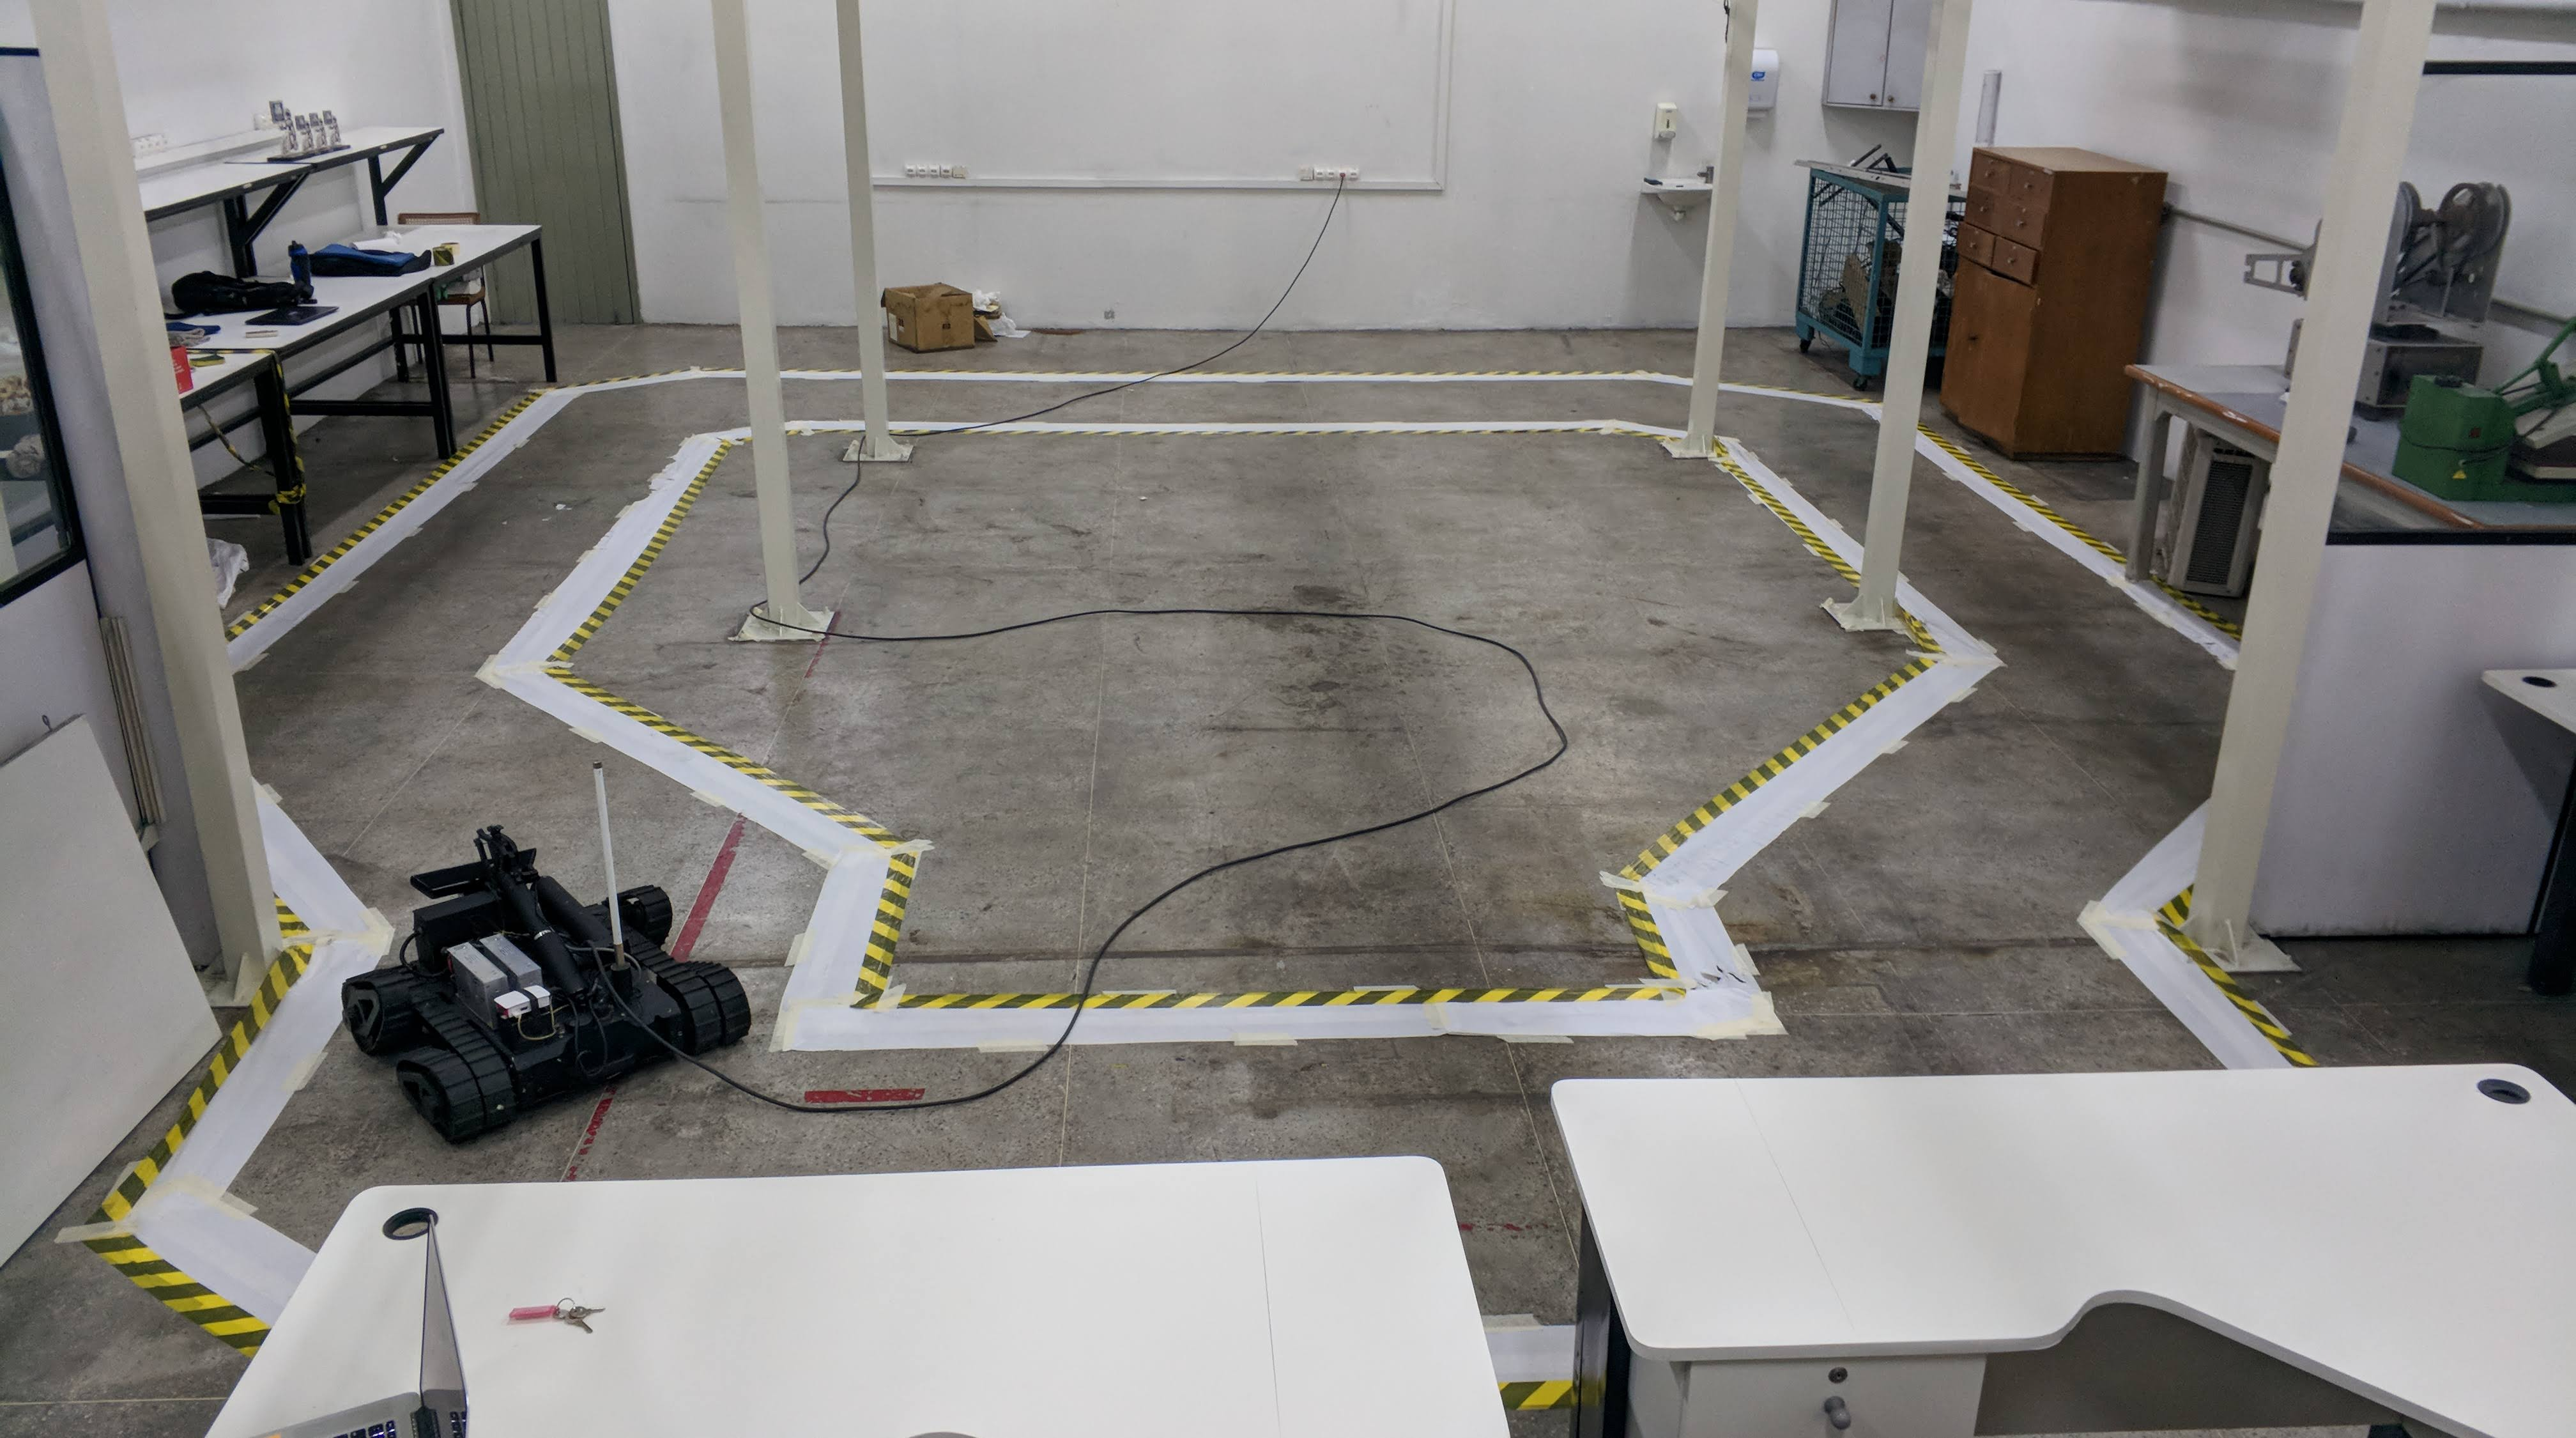
\includegraphics[width=15cm]{figuras/pista3.jpg}}
		}{
			\Fonte{Elaborado pelo autor}
		}	
\end{figure}

	\begin{figure}[H]
		\centering
		\Caption{\label{imagem3} Imagem Capturada pela câmera do Jaguar}
		\UNIFORfig{}{
			\fbox{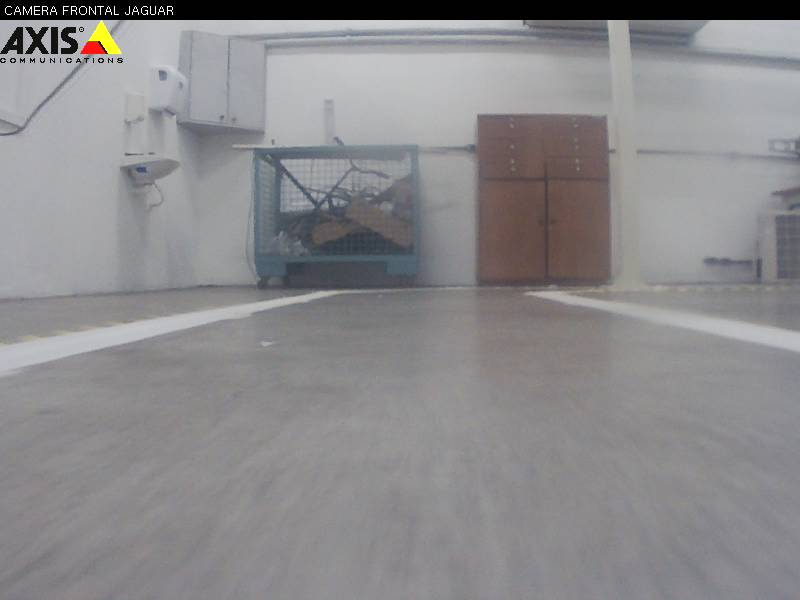
\includegraphics[width=15cm]{figuras/pista3imagemruim.jpg}}
		}{
			\Fonte{Elaborado pelo autor}
		}	
\end{figure}

Para o ultimo caso, a rede neural foi configurada com os parâmetros da tabela \ref{tabela2}:

\begin{table}[H]
\centering
\caption{Parâmetros de treinamento do segundo modelo}
\label{tabela2}
\begin{tabular}{|l|l|l|}
\hline
nb\_epoch & samples\_per\_epoch & batch\_size \\ \hline
20        & 2000                & 200         \\
20        & 5000                & 150         \\
20        & 10000               & 150         \\
30        & 20000               & 150         \\ \hline
\end{tabular}
\end{table}

Como o número de \textit{epoch} chega ao máximo de 30, poderá haver 30 modelos diferentes, mas não foi isso o que aconteceu. Como o programa está configurado para criar um modelo somente se ele tiver o \textit{val\_loss} menor que o anterior, nem sempre haverá a mesma quantidade de modelos para a quantidade de \textit{epoch} configurada. O programa fez um treinamento para cada \textit{epoch}, mas não gerou um modelo para cada um. Nesse caso foram apenas 16 modelos, nos quais os modelos 000, 001 e 013 se sairam melhor na segunda pista.

Para se chegar a um resultado satisfatório, era preciso que o Jaguar percorresse de forma autônoma pelo menos uma das pistas e boa parte da outra. Ele conseguiu fazer isso perfeitamente na primeira pista e boa parte da segunda, como é mostrado no video. Todos os arquivos do projeto podem ser encontrados no \textit{link} do \textit{GitHub} \cite{github}, assim como os video no link do \textit{YouTube} \cite{Youtube}.